\documentclass{report}
\usepackage{graphicx}
\usepackage{authblk}
\usepackage{amsmath}
\usepackage{listings}
\usepackage{subfigure}
\usepackage{algorithm2e}
\usepackage{minted}
\usepackage{booktabs}
\usepackage{float}
\usepackage{enumitem}
\usepackage{multirow}
\usepackage{diagbox}
\usepackage{subfigure}
\usepackage{pgfplots}


\title{ME 489\\ Homework 6 - CUDA Implementation of Obtaining Mandelbrot Set with Iterative Relations}

\author{Ata Bora Çakmakcı}
\author{Mustafa Yiğit Görgün}

\affil{Middle East Technical University}
\date{17 January 2024}

\begin{document}
\maketitle
\tableofcontents
\chapter{Introduction}
In this study we tried to find the complex numbers where the following conditions are satisfied:
$$
\left\{\begin{array}{l}
z_0=0 \\
z_{n+1}=z_n^2+c
\end{array}\right.
$$
To implement it both for C and for CUDA the following iterative relation was implemented for our use:
$$
x_{n+1}=x_n^2-y_n^2+x_0, \quad \text { and } \quad y_{n+1}=-2 x_n y_n+y_0 \text {. }
$$
Where the \emph{x} values denote the real part of the complex number \emph{c} and the \emph{y} values denote the imaginary part of \emph{c}. The visualization of the results (the points in the Mandelbrot set) can be seen in the Figure [BURAYA REF VE FIGURE KOY]. All "colored" points, which are not black, are the part of the Mandelbrot set where the black points are \emph{probably} not. The need to use probably in the earlier sentence is due to the number of iterations having a ceiling of a thousand in the creation of this image meaning we are not 100\% sure that they are not in the Mandelbrot set but we know that they did not make it into the set in the limit of given iterations. The colors are chosen with respect to the number of iterations required to find that point is included in the set. As the colors go from blue to green to red the number of iterations increase.
Throughout the implementation and elapsed time measurement of CUDA we used NVIDIA T4 GPU supplied by the Google Colab.

\chapter{Implementations}
\section{General CUDA Implementations}
Firstly we allocated enough memory, which is the total number of pixels, to the DEVICE array using \emph{cudaMalloc} function. Then we set the number of threads per thread block. Lastly we converted the number of threads per thread block and number of thread blocks to \emph{dim3} type integer. This is the accepted form of integer when launching a compute kernel in the triple chevrons which is the way we chose the launch the kernel instead of \emph{cudaLaunchKernel}. 
Secondly we changed the method of measuring time elapsed from calling \emph{clock()} functions to creating and starting cuda events then measuring time elapsed between them.
Lastly we called the \emph{mandelbrot} CUDA kernel with triple chevrons then copied the DEVICE array to the HOST array with \emph{cudaMemcpy}. We finished it off with freeing the DEVICE memory with \emph{cudaFree}.
\section{mandelbrot function}
We start off with making this function a CUDA kernel by including \emph{\_\_global\_\_} before the \emph{void} clause. The series version of this function included a nested for loop in order to call \emph{testpoint} function for every pixel in the given range. With CUDA implementation we got rid of this nested for loop since we identified each of the pixels by utilizing their thread and block IDs, already supplied by the CUDA, as following:
\begin{minted}{c}
    int t= threadIdx.x;
    int b= blockIdx.x;
    int B = blockDim.x;
    int n = t + b*B;
\end{minted}
\pagebreak
Even though, we were able to assign each pixel a distinct index these indices are not calculated with respect to these pixels' x and y coordinates. To determine the x and y coordinates we implemented the following calculations:
\begin{minted}{c}
    int nx= n%Nre;
    int ny= (n-n%Nre)/Nre;
\end{minted}
We now know the x and y coordinates of the given point with respect to our given bounds. Before we move on to constructing the complex number \emph{c} we have to ensure that our current coordinates are inside the specified bounds since if the total number of pixels are not a multiple of the number of threads in a thread block we may have threads with \emph{n} indices that are outside of the bounds. We ensure this by calling the \emph{testpoint} function inside the following if statement:
\begin{minted}{c}
  if (n<Nre*Nim){
    c.x=cmin.x+dc.x*nx;
    c.y=cmin.y+dc.y*ny;
    count[n] = (float )testpoint(c);   
  }
\end{minted}

\section{testpoint function}
The only implementation needed to be done on this function was to add \emph{\_\_device\_\_} before the \emph{int} clause to make it a DEVICE function, in other words, to let DEVICE be able to call this function.

\chapter{Results and Discussion}
\section{Results}
Since the code visualizes data itself no post-process was needed. The evolution of the output images of the code with increasing resolutions can be seen in the Figure \ref{fig:res_evo}. Since due to the limitations of the the \emph{.pdf} format the change is not really obvious hence we added a closeup version of all of these images in Figure \ref{fig:res_evo_close}.
\begin{figure}[H]
\begin{center}
\subfigure[]{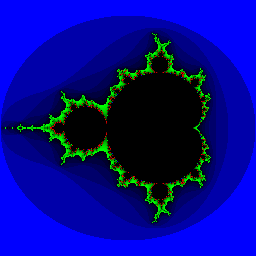
\includegraphics[height=1.8in,width=1.8in,angle=0]{figures/mandelbrot_256.png}}
\subfigure[]{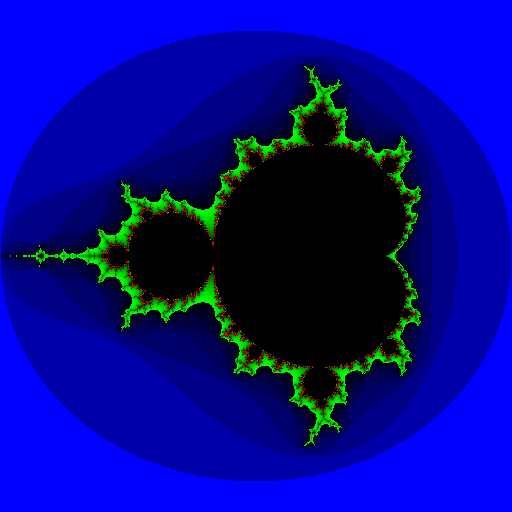
\includegraphics[height=1.8in,width=1.8in,angle=0]{figures/mandelbrot_512.png}}
\subfigure[]{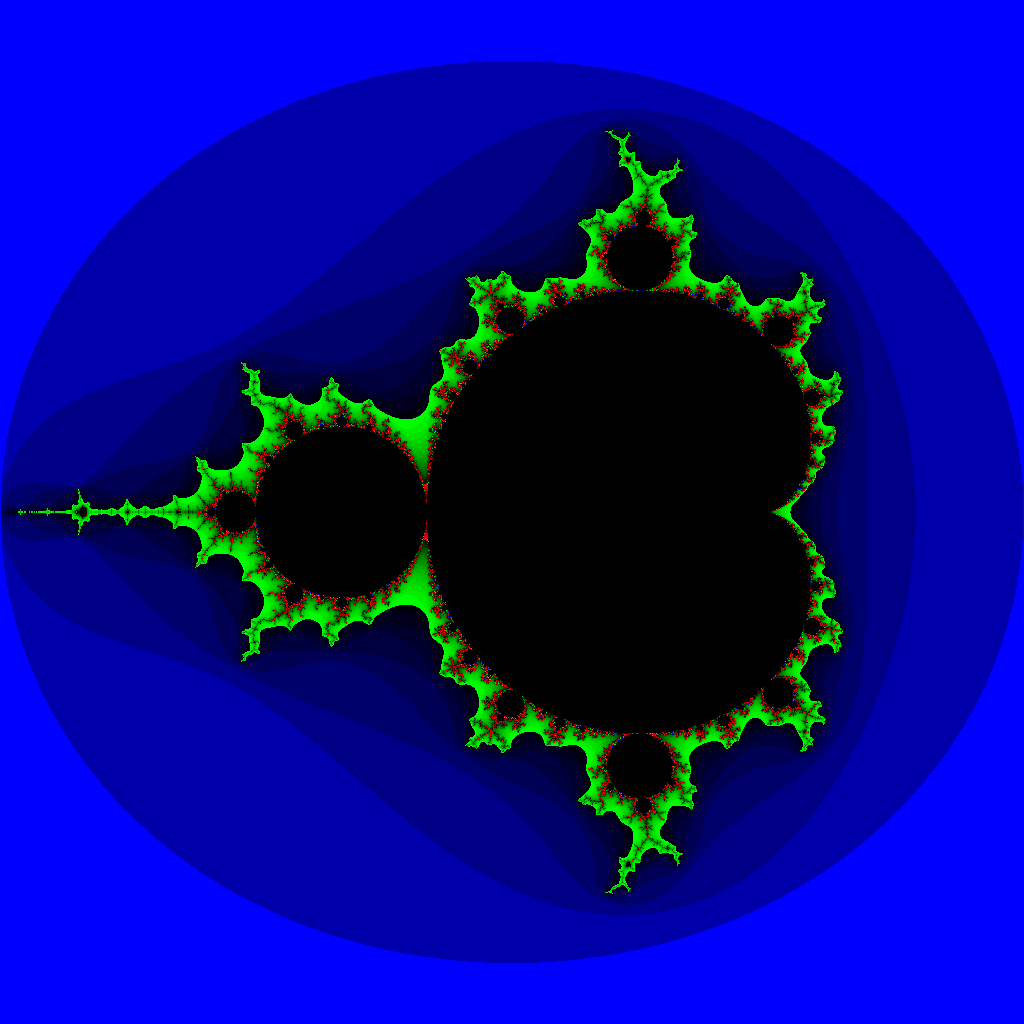
\includegraphics[height=1.8in,width=1.8in,angle=0]{figures/mandelbrot_1024.png}}
\subfigure[]{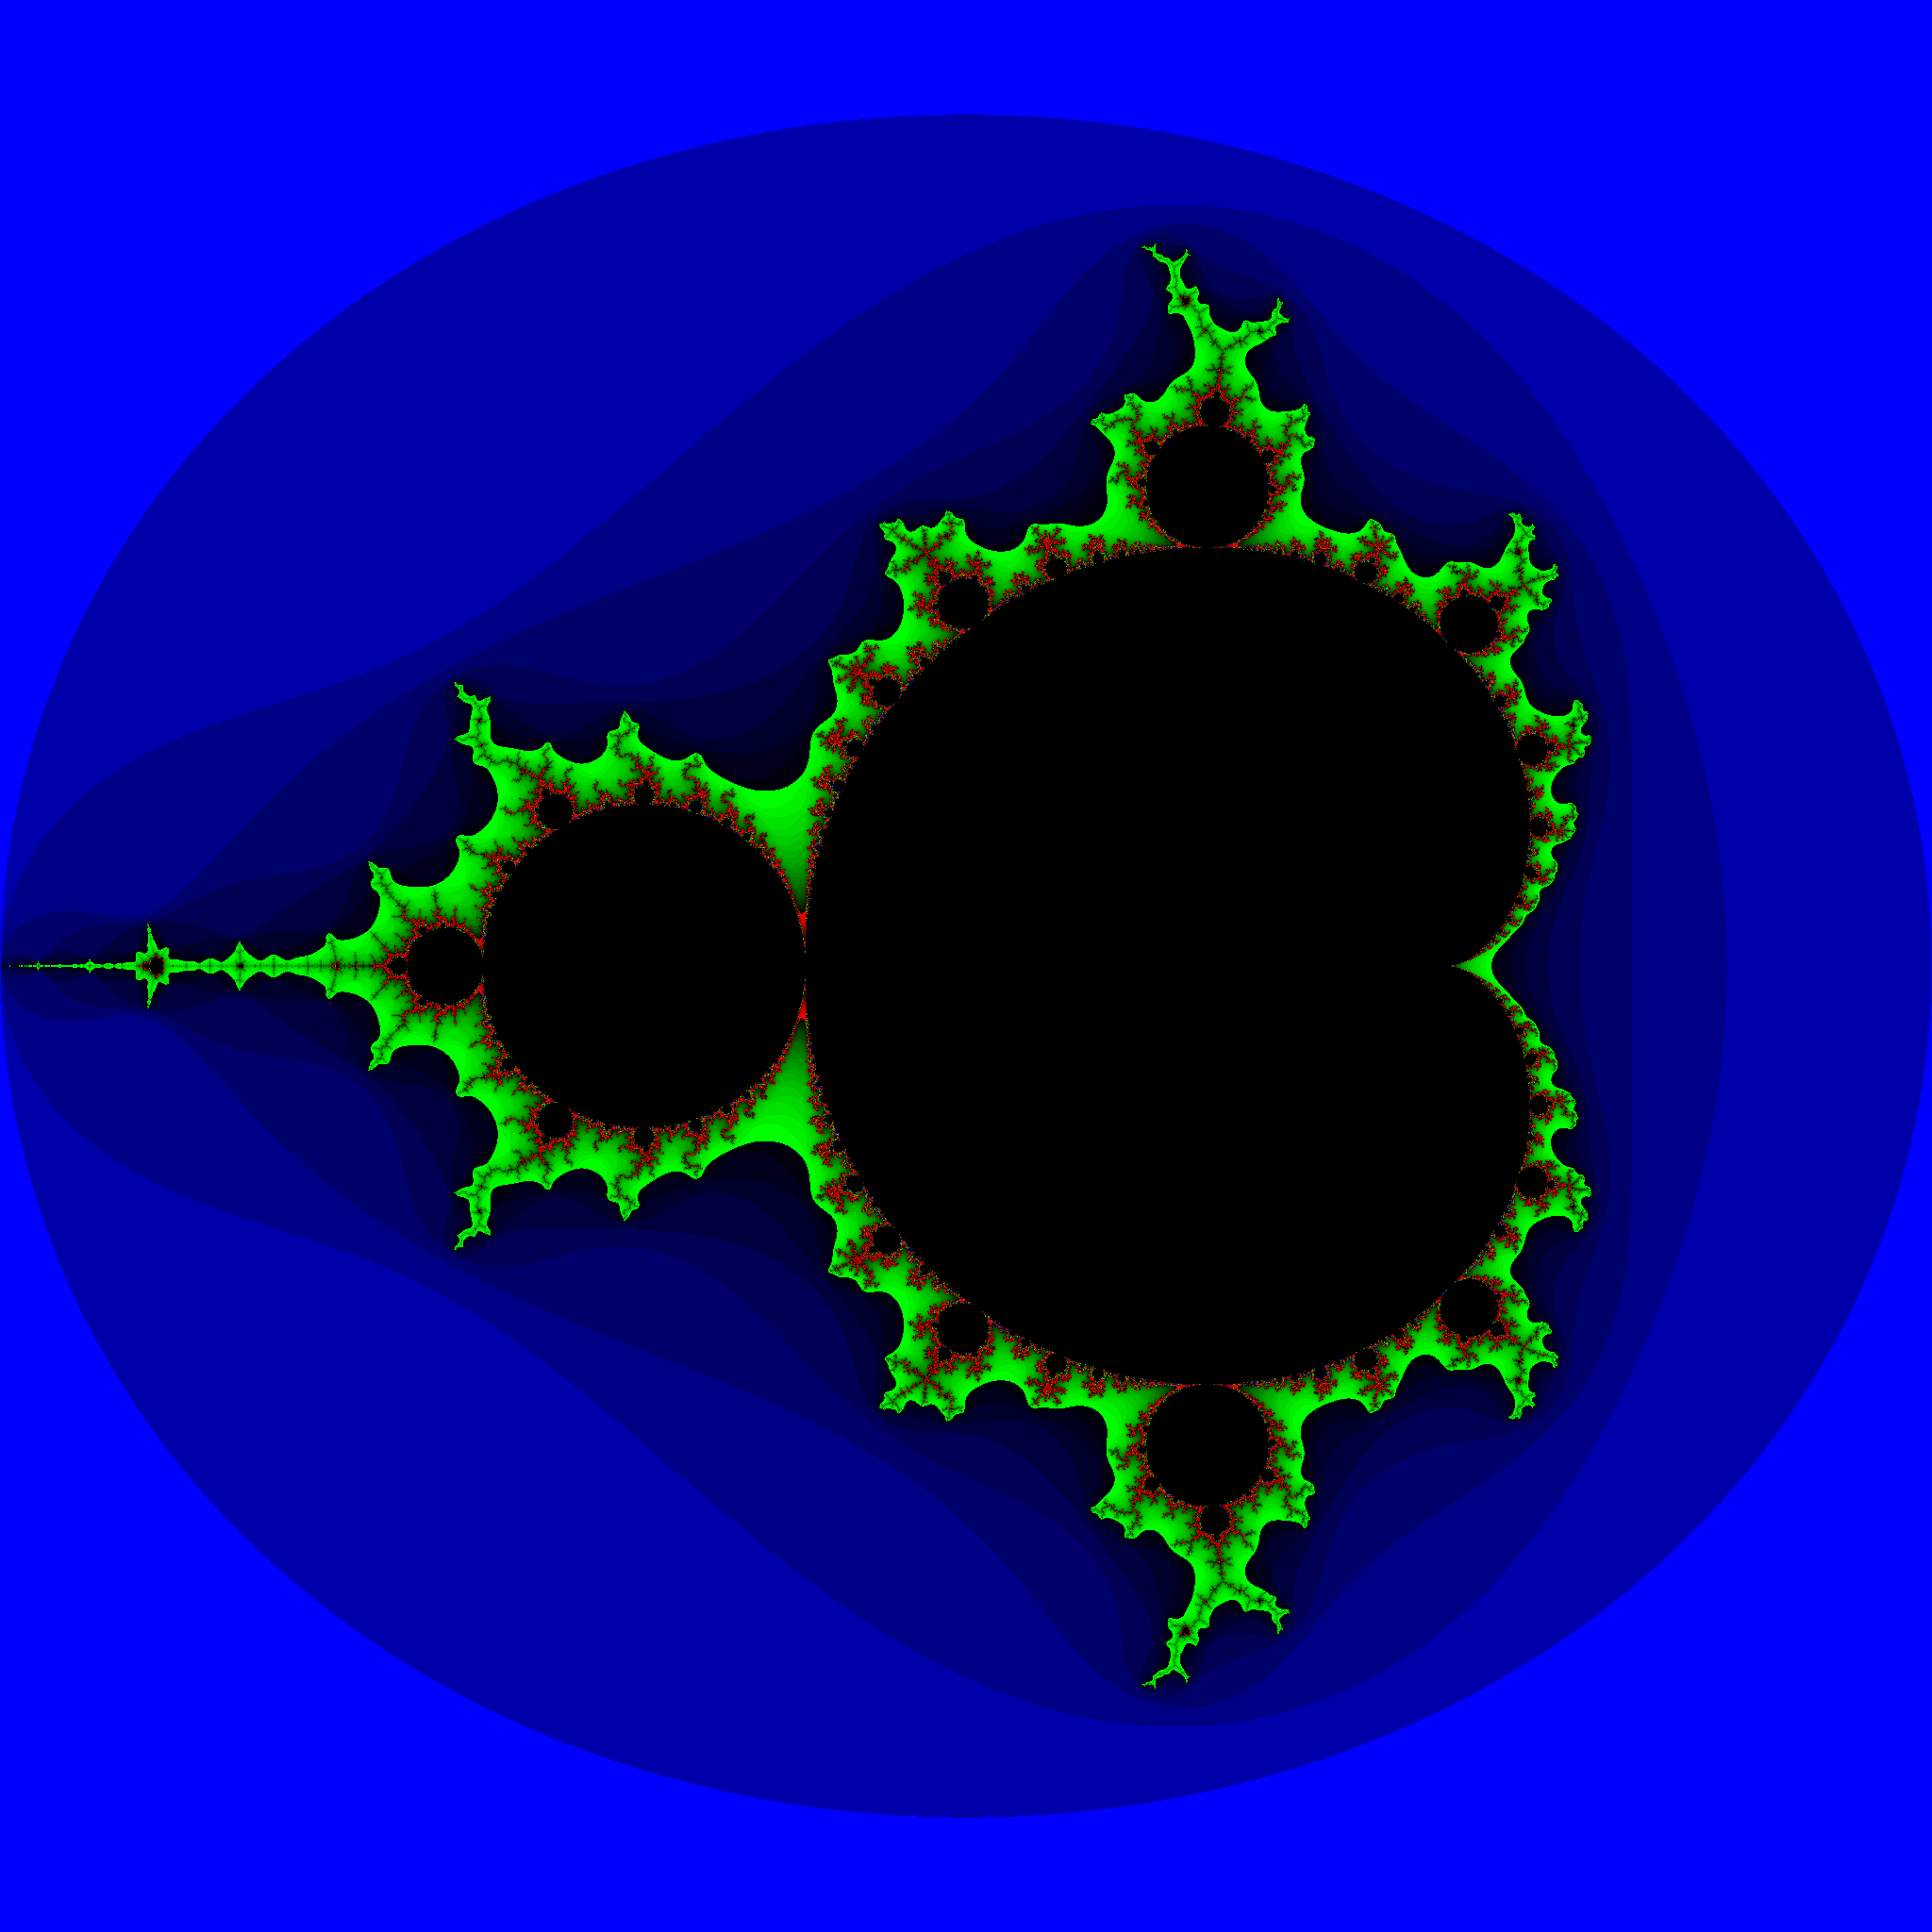
\includegraphics[height=1.8in,width=1.8in,angle=0]{figures/mandelbrot_2048.png}}
\subfigure[]{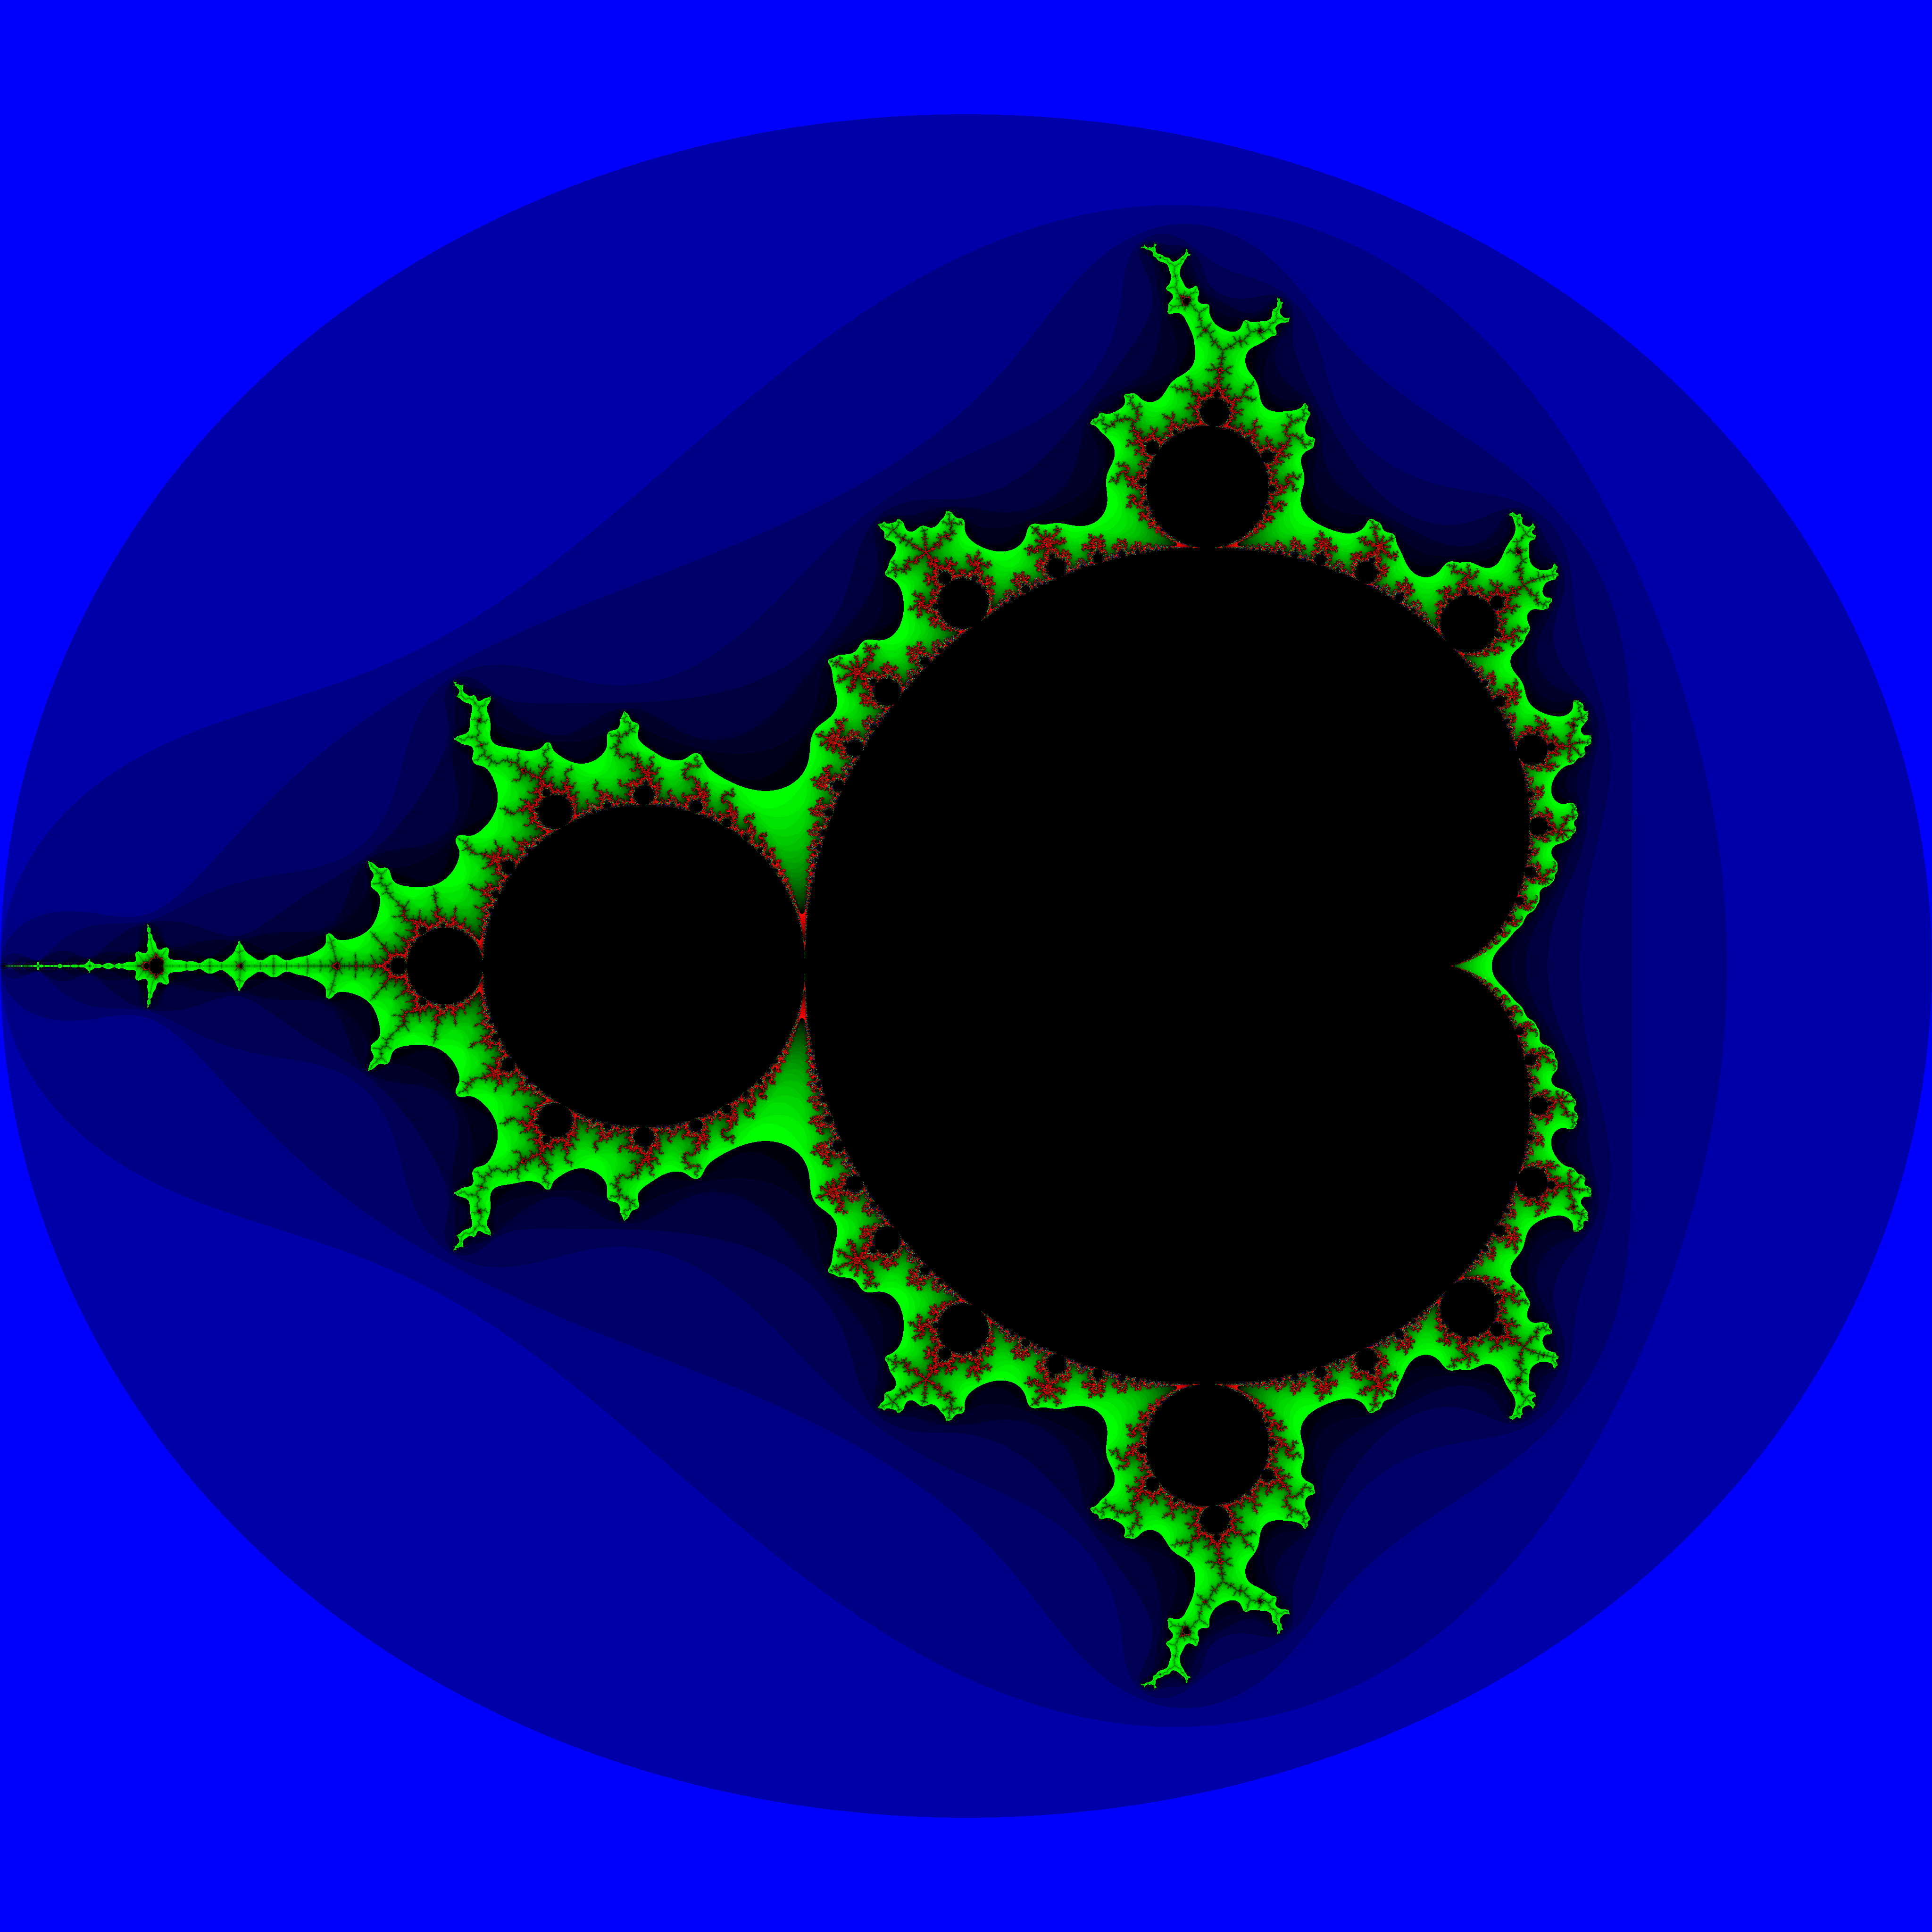
\includegraphics[height=1.8in,width=1.8in,angle=0]{figures/mandelbrot_4096.png}}
\subfigure[]{\includegraphics[height=1.8in,width=1.8in,angle=0]{figures/mandelbrot_8192.png}}
\subfigure[]{\includegraphics[height=1.8in,width=1.8in,angle=0]{figures/mandelbrot_16384.png}}
\caption{Visualization of Mandelbrot set with increasing number of resolutions of (a) 256*256 (b) 512*512 (c) 1024*1024 (d) 2048*2048 (e) 4096*4096 (f) 8192*8192 (g) 16384*16384}
\label{fig:res_evo}
\end{center}
\end{figure}
\begin{figure}[H]
\begin{center}
\subfigure[]{
\includegraphics[height=1.8in,width=1.8in,angle=0]{figures/closeup_256.png}}
\subfigure[]{
\includegraphics[height=1.8in,width=1.8in,angle=0]{figures/closeup_512.png}}
\subfigure[]{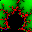
\includegraphics[height=1.8in,width=1.8in,angle=0]{figures/closeup_1024.png}}
\subfigure[]{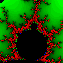
\includegraphics[height=1.8in,width=1.8in,angle=0]{figures/closeup_2048.png}}
\subfigure[]{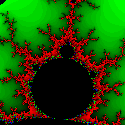
\includegraphics[height=1.8in,width=1.8in,angle=0]{figures/closeup_4096.png}}
\subfigure[]{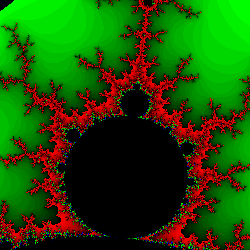
\includegraphics[height=1.8in,width=1.8in,angle=0]{figures/closeup_8192.png}}
\subfigure[]{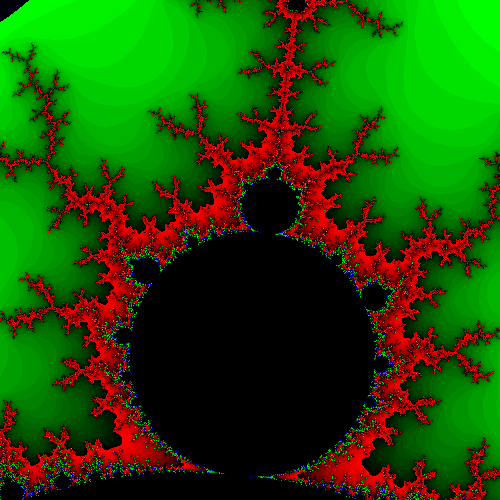
\includegraphics[height=1.8in,width=1.8in,angle=0]{figures/closeup_16384.png}}
\caption{Closeup view of the visualization of Mandelbrot set with increasing number of resolutions of (a) 256*256 (b) 512*512 (c) 1024*1024 (d) 2048*2048 (e) 4096*4096 (f) 8192*8192 (g) 16384*16384 for the same portion of the total image}
\label{fig:res_evo_close}
\end{center}
\end{figure}
\pagebreak
\pagebreak
\\
We measured the time taken for both series and CUDA implemented versions of the code with different resolutions. We ran the code multiple times to obtain an average.
\begin{table}[h]
    \centering
    \hspace*{-3cm}\begin{tabular}{|c|c|c|c|}
        \hline
        Resolution & Series Version Time Elapsed(s) & CUDA Implementation Time Elapsed (s) & Ammount of Speed Up \\
        \hline
        256*256 & 0.029890 &0.005111 & 5.848\\
        \hline
        512*512 & 0.111800 &0.014453 & 7.740\\
        \hline
        1024*1024 & 0.436373 &0.046790 & 9.326\\
        \hline
        2048*2048 & 1.737644 & 0.163506 & 10.627\\
        \hline
        4096*4096 & 7.039794 & 0.439807 & 16.007 \\
        \hline
        8192*8192 & 28.411598 & 1.262110 & 22.511\\
        \hline
        16384*16384 & 112.894022 & 4.562895 & 24.742\\
        \hline
    \end{tabular}
    \caption{Elapsed time(s) and speed up amounts for Series and CUDA implemented versions of the code of different resolutions.}
    \label{table1}
\end{table}



\newpage
\section{Discussion}
\paragraph{}
As can be seen from the Figure \ref{fig:res_evo_close}, resolutions below a certain threshold give results that are less accurate in determining the points that belongs to the Mandelbrot set. On the other hand, increased resolutions naturally increase the computational load, which results in considerably longer computation times as can be seen in Table \ref{table1}. Any application that will reduce this time is very valuable, and the way we were prompted to choose, CUDA has been applied in this project. Our code, which was extended to run on the GPU via CUDA, was run on T4 GPUs via Google Colab.

\paragraph{}
The time elapsed data in Table \ref{table1} shows that the elapsed times increase \emph{almost} linearly with the resolutions. Both, series and CUDA implemented codes elapsed times increase with factors of \emph{nearly} 4 as the resolution also goes up by a factor of 4. The need for "\emph{nearly}" and "\emph{almost}" is that this does not transform well into the amount of speed up that can be seen in the same table. This effect is due to the non-linear relationship between the resolution and the time elapsed for both versions of the code. Even though, at first they seem to be increasing by factors of 4 they are actually increasing with different factors at different resolutions and since, as expected, the more load on series will slow down the code more than the increase in resolution and as the resolution becomes larger more GPU threads will be implemented with CUDA. As a result time spent on data transfer and serial calculations decreases, and the computational weight shifts to the parallel operating CUDA threads.
\end{document}